\documentclass[12pt]{article}
\author{Matthew D. Cocci}
\title{Homework 9}
\date{\today}
%% Formatting & Spacing %%%%%%%%%%%%%%%%%%%%%%%%%%%%%%%%%%%%

%\usepackage[top=1in, bottom=1in, left=1in, right=1in]{geometry} % most detailed page formatting control
\usepackage{fullpage} % Simpler than using the geometry package; std effect
\usepackage{setspace}
%\onehalfspacing
\usepackage{microtype}


%% Header %%%%%%%%%%%%%%%%%%%%%%%%%%%%%%%%%%%%%%%%%%%%%%%%%

%\usepackage{fancyhdr}
%\pagestyle{fancy}
%\lhead{}
%\rhead{}
%\chead{}
%\setlength{\headheight}{15.2pt}
    %---Make the header bigger to avoid overlap

%\renewcommand{\headrulewidth}{0.3pt}
    %---Width of the line

%\setlength{\headsep}{0.2in}
    %---Distance from line to text


%% Mathematics Related %%%%%%%%%%%%%%%%%%%%%%%%%%%%%%%%%%%

\usepackage{amsmath}
\usepackage{amsfonts}
\usepackage{mathrsfs}
\usepackage{amsthm} %allows for labeling of theorems
\theoremstyle{plain}
\newtheorem{thm}{Theorem}[section]
\newtheorem{lem}[thm]{Lemma}
\newtheorem{prop}[thm]{Proposition}
\newtheorem{cor}[thm]{Corollary}

\theoremstyle{definition}
\newtheorem{defn}[thm]{Definition}
\newtheorem{ex}[thm]{Example}

\theoremstyle{remark}
\newtheorem*{rem}{Remark}
\newtheorem*{note}{Note}

% Below supports left-right alignment in matrices so the negative
% signs don't look bad
\makeatletter
\renewcommand*\env@matrix[1][c]{\hskip -\arraycolsep
  \let\@ifnextchar\new@ifnextchar
  \array{*\c@MaxMatrixCols #1}}
\makeatother


%% Font Choices %%%%%%%%%%%%%%%%%%%%%%%%%%%%%%%%%%%%%%%%%

\usepackage[T1]{fontenc}
\usepackage{lmodern}
\usepackage[utf8]{inputenc}
%\usepackage{blindtext}


%% Figures %%%%%%%%%%%%%%%%%%%%%%%%%%%%%%%%%%%%%%%%%%%%%%

\usepackage{graphicx}
\usepackage{subfigure}
    %---For plotting multiple figures at once
%\graphicspath{ {Directory/} }
    %---Set a directory for where to look for figures


%% Hyperlinks %%%%%%%%%%%%%%%%%%%%%%%%%%%%%%%%%%%%%%%%%%%%
\usepackage{hyperref}
\hypersetup{
    colorlinks,
        %---This colors the links themselves, not boxes
    citecolor=black,
        %---Everything here and below changes link colors
    filecolor=black,
    linkcolor=black,
    urlcolor=black
}

%% Including Code %%%%%%%%%%%%%%%%%%%%%%%%%%%%%%%%%%%%%%%

\usepackage{verbatim}
    %---For including verbatim code from files, no colors

\usepackage{listings}
\usepackage{color}
\definecolor{mygreen}{RGB}{28,172,0}
\definecolor{mylilas}{RGB}{170,55,241}
\newcommand{\matlabcode}[1]{%
    \lstset{language=Matlab,%
        basicstyle=\footnotesize,%
        breaklines=true,%
        morekeywords={matlab2tikz},%
        keywordstyle=\color{blue},%
        morekeywords=[2]{1}, keywordstyle=[2]{\color{black}},%
        identifierstyle=\color{black},%
        stringstyle=\color{mylilas},%
        commentstyle=\color{mygreen},%
        showstringspaces=false,%
            %---Without this there will be a symbol in
            %---the places where there is a space
        numbers=left,%
        numberstyle={\tiny \color{black}},%
            %---Size of the numbers
        numbersep=9pt,%
            %---Defines how far the numbers are from the text
        emph=[1]{for,end,break,switch,case},emphstyle=[1]\color{red},%
            %---Some words to emphasise
    }%
    \lstinputlisting{#1}
}
    %---For including Matlab code from .m file with colors,
    %---line numbering, etc.

%% Bibliographies %%%%%%%%%%%%%%%%%%%%%%%%%%%%%%%%%%%%

%\usepackage{natbib}
    %---For bibliographies
%\setlength{\bibsep}{3pt} % Set how far apart bibentries are

%% Misc %%%%%%%%%%%%%%%%%%%%%%%%%%%%%%%%%%%%%%%%%%%%%%

\usepackage{enumitem}
    %---Has to do with enumeration
\usepackage{appendix}
\usepackage{pdfpages}
    %---For including whole pdf pages as a page in doc


%% User Defined %%%%%%%%%%%%%%%%%%%%%%%%%%%%%%%%%%%%%%%%%%

%\newcommand{\nameofcmd}{Text to display}



%%%%%%%%%%%%%%%%%%%%%%%%%%%%%%%%%%%%%%%%%%%%%%%%%%%%%%%%%%%%%%%%%%%%%%%%
%% BODY %%%%%%%%%%%%%%%%%%%%%%%%%%%%%%%%%%%%%%%%%%%%%%%%%%%%%%%%%%%%%%%%
%%%%%%%%%%%%%%%%%%%%%%%%%%%%%%%%%%%%%%%%%%%%%%%%%%%%%%%%%%%%%%%%%%%%%%%%


\begin{document}
\maketitle

%\tableofcontents


\begin{enumerate}
  \item % Question 1
    \begin{enumerate}
      \item % Question 1a
        We want to compute the following
        \begin{align*}
          \int^t_0 \int_0^{s_1} \int_0^{s_2} dW_{s_3}dW_{s_2}dW_{s_1}
          &= \int^t_0 \int_0^{s_1} (W_{s_2}-W_0)dW_{s_2}dW_{s_1}\\
          &= \int^t_0 \int_0^{s_1} W_{s_2}dW_{s_2}dW_{s_1}
        \end{align*}
        We saw before in class that $\int^t_0 W_s dW_s =
        \frac{1}{2}(W_t^2-t)$, hence
        \begin{align*}
          \int^t_0 \int_0^{s_1} \int_0^{s_2} dW_{s_3}dW_{s_2}dW_{s_1}
          &= \int^t_0 \int_0^{s_1} W_{s_2}dW_{s_2}dW_{s_1}\\
          &= \int^t_0 \frac{1}{2}\left(
              W_{s_1}^2 - s_1
              \right)dW_{s_1}\\
          &= \frac{1}{2}\int^t_0 W_{s_1}^2 dW_{s_1}
              -\frac{1}{2} \int^t_0s_1 dW_{s_1}
        \end{align*}
        In the a previous homework, we also saw that $\int^t_0 W_s^2
        dW_s = \frac{1}{3}W_t^3 - \int^t_0 W_s ds$, allowing us to
        simplify further
        \begin{align}
          \int^t_0 \int_0^{s_1} \int_0^{s_2} dW_{s_3}dW_{s_2}dW_{s_1}
          &= \frac{1}{2}\int^t_0 W_{s_1}^2 dW_{s_1}
              -\frac{1}{2} \int^t_0s_1 dW_{s_1}\notag\\
          &= \frac{1}{2}\left(\frac{1}{3}W_t^3 - \int^t_0 W_s ds\right)
              -\frac{1}{2} \int^t_0s_1 dW_{s_1}\notag\\
          &= \frac{1}{6}W_t^3 - \frac{1}{2}\int^t_0 W_s ds
            -\frac{1}{2} \int^t_0s_1 dW_{s_1} \label{q1a.1}
        \end{align}
        Now, we want to simplify the integrals in
        Expression~\ref{q1a.1}. To simplify the integral $\int^t_0 s_w
        dW_{s_1}$, we will use Ito's Lemma. So suppose that we have
        \begin{align*}
          X_t = W_t \qquad &\Leftrightarrow \qquad dX_t = dW_t \\
          f(t,x) = tx \qquad &\Rightarrow \qquad
          \frac{\partial f}{\partial t} = x
          \qquad \frac{\partial f}{\partial x} = t
          \qquad \frac{\partial^2 f}{\partial x^2} = 0
        \end{align*}
        To see why $f(t,x)=tx$ is an appropriate choice, see the
        appendix attached at the end of this homework, which is included
        for completeness.

        Applying Ito's Lemma:
        \begin{align*}
          d\left(tX_t\right)
            &= \frac{\partial f}{\partial t} dt
              + \frac{\partial f}{\partial x} dX_t
              + \frac{1}{2} \frac{\partial^2 f}{\partial x^2} (dX_t)^2\\
            &= X_t dt + t dX_t + 0
        \end{align*}
        Substituting in $X_t = W_t$ and $dX_t = dW_t$, we get
        \begin{align*}
          d\left(tW_t\right) &= W_t dt + t dW_t
        \end{align*}
        Integrating gives
        \begin{align}
          \int^t_0 d\left(sW_s\right) &= \int^t_0 W_s ds + \int^t_0 s dW_s
          \notag \\
          \Rightarrow \qquad
          tW_t &= \int^t_0 W_s ds + \int^t_0 s dW_s\notag \\
          \Rightarrow \qquad
          \int^t_0 s dW_s &=
            tW_t - \int^t_0 W_s ds
            \label{q1a.2}
        \end{align}
        Substituting this result into Expression~\ref{q1a.1}, we get
        \begin{align*}
          \int^t_0 \int_0^{s_1} \int_0^{s_2} dW_{s_3}dW_{s_2}dW_{s_1}
          &= \frac{1}{6}W_t^3 - \frac{1}{2}\int^t_0 W_s ds
            -\frac{1}{2} \left(
              tW_t - \int^t_0 W_{s_1} ds_1
            \right) \\
          &= \frac{1}{6}W_t^3 -\frac{1}{2} tW_t
        \end{align*}

      \item % Question 1b
        Since we need to use $I^{(k-2)}$ in the induction formula, let's
        proceed by first proving that moving from $k=2$ to $k=3$ holds.
        To do so, we'll need to examing the cases where $k=1,2,3$.

        For $k=1$:
        \begin{align*}
          \int^t_0 dW_s = W_t
        \end{align*}

        For $k=2$:
        \begin{align*} I^{(2)}_t
          &= \int^t_0 dW_{s_1} \int^{s_1}_0 dW_{s_2}\\
          &= \int^t_0 W_{s_1} dW_{s_1} \\
          &= \frac{1}{2}(W_t^2 - t)
        \end{align*}

        For $k=3$, we use the result from Part 1a:
        \begin{align*}
          I^{(3)}_t
          &= \int^t_0 dW_{s_1} \int^{s_1}_0 dW_{s_2} \int^{s_2}_0 dW_{s_3}\\
          &=\int^t_0\int^{s_1}_0\int^{s_2}_0 dW_{s_3} dW_{s_2} dW_{s_1} \\
          &= \frac{1}{6} W_t^3 - \frac{1}{2} tW_t
        \end{align*}

        Now, substituting into the induction formula for $k=3$ to check,
        we see
        \begin{align*}
          \frac{1}{3}\left(W_t I^{(2)}_t - tI^{(1)}_t\right)
          &=
          \frac{1}{3}\left(W_t \left[ \frac{1}{2}(W_t^2 - t)\right]
              - tW_t\right)\\
          &=
          \frac{1}{3}\left( \frac{1}{2}W_t^3 - \frac{1}{2}tW_t
              - tW_t\right)\\
          &=
          \frac{1}{3}\left( \frac{1}{2}W_t^3 - \frac{3}{2}tW_t\right)\\
          &=
          \frac{1}{6}W_t^3 - \frac{1}{2}tW_t
          = I^{(3)}_t
        \end{align*}

      \item From there, I wasn't able to get the induction step to work.

        %So it checks out. Now assume that the case holds for $k$. We
        %want to prove $k+1$. Therefore, write out the $k+1$ integration
        %problem as follows:
        %\begin{align*}
          %\int^t_0 dW_{s_1} \int^{s_1}_0 dW_{s_2}
          %\cdots \int^{s_{k-1}}_0 dW_{s_{k}}
          %\int^{s_k}_0 dW_{s_{k+1}}
        %\end{align*}
        %Now rearrange as we did above into something that looks like the
        %form we saw in Q1a:
        %\begin{align*}
          %\int^t_0 \int^{s_1}_0 \cdots \int^{s_{k-1}}_0
          %\int^{s_k}_0 dW_{s_{k+1}} dW_{s_{k}}\cdots
          %dW_{s_2}dW_{s_1}
        %\end{align*}
        %Simplifying the middle integral:
        %\begin{align*}
          %\int^t_0 \int^{s_1}_0 \cdots \int^{s_{k-1}}_0
          %W_{s_{k}}dW_{s_{k}}\cdots
          %dW_{s_2}dW_{s_1}
        %\end{align*}

    \end{enumerate}

  \clearpage
  \item % Question 2
    First, the identity that will be heavily used
    \begin{align}
      f(X_t) &= f(X_0) + \int^t_0 \mathscr{L}_0 f(X_s) ds
      +\int^t_0 \mathscr{L}_1 f(X_s) dW_s
      \label{q2.1}\\
      \mathscr{L}_0
        &= b\frac{\partial}{\partial x}
          +\frac{1}{2}\sigma^2\frac{\partial^2}{\partial x^2}
        \qquad\qquad
      \mathscr{L}_1 = \sigma \frac{\partial}{\partial x}
      \notag
    \end{align}
    To get to the Milstein scheme, we considered the first remainder
    from Ito expansion:
    \begin{align}
      \label{q2.2}
      R_1
      &=
      \int^t_0 \int^s_0 \mathscr{L}_0b(X_z) dz ds
      +\int^t_0 \int^s_0 \mathscr{L}_1 b(X_z) dW_z ds
      +\int^t_0 \int^s_0 \mathscr{L}_0 \sigma(X_z) dz dW_s\\
      &\qquad
      +\int^t_0 \int^s_0 \mathscr{L}_1 \sigma(X_z) dW_z dW_s
      \notag
    \end{align}
    From there, we only expanded the last term.  So let's now expand the
    other double integrals.
    \begin{enumerate}
      \item First, we apply (\ref{q2.1}), taking $f=\mathscr{L}_0b(X_s)$
        \begin{align*}
          \int^t_0 \int^s_0 \mathscr{L}_0b(X_z) dz ds
          &=
          \int^t_0 \int^s_0 \left[
            \mathscr{L}_0b(X_0)
            + \int^p_0 \mathscr{L}_0^2b(X_z) dp
            + \int^p_0 \mathscr{L}_1\mathscr{L}_0b(X_z) dW_p
            \right] dz ds \\
          &=
          \mathscr{L}_0b(X_0)
            \int^t_0 \int^s_0 dz ds
            + \int^t_0 \int^s_0\int^p_0 \mathscr{L}_0^2b(X_z) dp dz ds\\
          &\qquad
            + \int^t_0 \int^s_0\int^p_0
              \mathscr{L}_1\mathscr{L}_0b(X_z) dW_p dz ds
        \end{align*}
        We'll drop the triple integral terms in the approximation,
        leaving
        \begin{align*}
          \int^t_0 \int^s_0 \mathscr{L}_0b(X_z) dz ds
          &\approx
          \mathscr{L}_0b(X_0) \int^t_0 \int^s_0 dz ds\\
          &=
          \mathscr{L}_0b(X_0) \frac{t^2}{2}\\
          &=
          \left[ b\frac{\partial}{\partial x} + \frac{1}{2}\sigma^2
          \frac{\partial^2}{\partial x^2}\right]
            b(X_0) \frac{t^2}{2}\\
          \Rightarrow \qquad
          \int^t_0 \int^s_0 \mathscr{L}_0b(X_z) dz ds
            &\approx \left( bb' + \frac{1}{2}\sigma^2 b''\right)
            \frac{t^2}{2}
        \end{align*}
        where $b$, $b'$, and $\sigma$ are all evaluated at $X_0$.

      \item Next, we expand the second term in (\ref{q2.2}), taking
        $f=\mathscr{L}_1b(X_z)$ in (\ref{q2.1}). If we do that and drop
        the triple integral terms, we'll be left with:
        \begin{align*}
          \int^t_0 \int^s_0 \mathscr{L}_1 b(X_z) dW_z ds
          &\approx
          \mathscr{L}_1 b(X_0)
          \int^t_0 \int^s_0 dW_z ds\\
          &=
          \sigma \frac{\partial}{\partial x}
          b(X_0)
          \int^t_0 \int^s_0 dW_z ds\\
          &=
          \sigma b' Z_t
        \end{align*}
        where $\sigma$ and $b'$ are evaluated at $X_0$ and
        \begin{align*}
          Z_t:=\int^t_0\int^s_0 dW_s ds
          \qquad
          Z_t \sim N(0,\frac{1}{3}t^3)
          \qquad EZ_t W_t = \frac{1}{2}t^2
        \end{align*}
        as given in the problem statement.

      \item Lastly, the third double integral in (\ref{q2.2}). If we
        expand and drop triple integrals, we get
        \begin{align*}
          \int^t_0 \int^s_0 \mathscr{L}_0 \sigma(X_z) dz dW_s
          &\approx
          \mathscr{L}_0 \sigma(X_0) \int^t_0 \int^s_0  dz dW_s\\
          &=
          \mathscr{L}_0 \sigma(X_0) \int^t_0 s \;dW_s
        \end{align*}
        Using a Result~(\ref{q1a.2}) from Question 1, we can simplify
        that integral
        \begin{align*}
          \int^t_0 \int^s_0 \mathscr{L}_0 \sigma(X_z) dz dW_s
          &\approx
          \mathscr{L}_0 \sigma(X_0) \int^t_0 s dW_s \\
          &=
          \mathscr{L}_0\sigma(X_0)\left(tW_t - \int^t_0 W_s ds\right)\\
          &=
          \mathscr{L}_0\sigma(X_0)
          \left(tW_t - \int^t_0 \int^s_0 dW_z ds\right)\\
          &=
          \mathscr{L}_0\sigma(X_0)\left(tW_t - Z_t\right)
        \end{align*}
        where I use the definition of $Z_t$ from above. Then, expanding
        out $\mathscr{L}_0\sigma(X_0)$, we get
        \begin{align*}
          \int^t_0 \int^s_0 \mathscr{L}_0 \sigma(X_z) dz dW_s
          &\approx
          \left(b\sigma' + \frac{1}{2}\sigma^2\sigma''\right)
          \left(tW_t - Z_t\right)
        \end{align*}
    \end{enumerate}
    Finally, the only thing left to do is expand out the triple-integral
    Ito term that was generated by the Milstein expansion and left in
    the remainder. Doing that by taking $f=\mathscr{L}_1^2\sigma(X_p)$
    (and dropping all quadruple integral terms) gives
    \begin{align*}
        \int^t_0\int^s_0 \int^z_0
          &\mathscr{L}^2_1\sigma(X_p) dW_p dW_z dW_s\\
      &=
        \int^t_0\int^s_0 \int^z_0
        \left[
          \mathscr{L}^2_1\sigma(X_0)
          +\int^p_0 \mathscr{L}_0 \mathscr{L}^2_1\sigma(X_q) dq
          +\int^p_0 \mathscr{L}^3_1\sigma(X_q) dW_q
        \right]
        dW_p dW_z dW_s\\
      &\approx
        \mathscr{L}^2_1\sigma(X_0) \int^t_0\int^s_0 \int^z_0 dW_p dW_z dW_s
    \end{align*}
    To simplify, compute the leading term
    \begin{align*}
      \mathscr{L}^2_1\sigma(X_0)
      &=
      \mathscr{L}_1\left(\mathscr{L}_1\sigma(X_0)\right) \\
      &=
      \mathscr{L}_1\left(
        \sigma
        \frac{\partial}{\partial x}\sigma(X_0)
      \right)
      = \mathscr{L}_1 \left( \sigma \sigma' \right) \\
      &=
      \sigma
        \frac{\partial}{\partial x}
      \left( \sigma \sigma' \right) \\
      &=
      \sigma
      \left(
        \sigma \sigma''
        + \left[\sigma'\right]^2
      \right) \\
      &=
        \sigma^2 \sigma''
        + \sigma\left[\sigma'\right]^2
    \end{align*}
    where $\sigma$, $\sigma'$, and $\sigma''$ are all evaluated at $X_0$.

    Finally, let's compute the integral, using the answer from Q1:
    \begin{align*}
        \int^t_0\int^s_0 \int^z_0 dW_p dW_z dW_s
        &= \frac{1}{6}W_t^3 - \frac{1}{2} t W_t \\
      \Rightarrow \qquad
        \mathscr{L}^2_1\sigma(X_0)
        \int^t_0\int^s_0 \int^z_0 dW_p dW_z dW_s
        &= \left( [\sigma(X_0)]^2 \sigma''(X_0)
        + \sigma(X_0)\left[\sigma'(X_0)\right]^2\right)
          \left(
          \frac{1}{6}W_t^3 - \frac{1}{2} t W_t\right)
    \end{align*}
    Putting everything together, this all suggests the following scheme:
    \begin{align*}
      X_{n+1}
        &= X_n
        + b\Delta t + \sigma \Delta W_n
        + \frac{1}{2}\sigma\sigma' ( (\Delta W_n)^2 - \Delta t)\\
      &\quad + \frac{1}{2}\left(bb'+\frac{1}{2}\sigma^2 b''\right)
        (\Delta t)^2\\
      &\quad + \sigma b' \Delta Z\\
      &\quad + \left( b\sigma' + \frac{1}{2}\sigma^2\sigma''\right)
      \left[(\Delta t) (\Delta W_t) -\Delta Z\right]\\
      &\quad+ \frac{1}{2}\left(\sigma^2\sigma'' +\sigma(\sigma')^2\right)
        \left(\frac{1}{3}(\Delta W_n)^2 -\Delta t
        \right)(\Delta W_n)
    \end{align*}
    where $b$, $b'$, $b''$, $\sigma$, $\sigma'$, and $\sigma''$ are all
    evaluated at $X_n$. To implement, we draw
    \begin{align*}
      \Delta W_n \sim N(0,\Delta t)
      \qquad
      \Delta Z \sim N\left(0,\frac{1}{3}(\Delta t)^3\right)
      \quad \text{where} \quad
      E[(\Delta Z)(\Delta W_n)] = \frac{1}{2}\Delta t
    \end{align*}


  \item % Question 3
    We want to compute analytically the region of mean-square stability
    of Geometric Brownian Motion $X_t$ for the Milstein scheme, where
    $X_t$ follows:
    \begin{align*}
      dX_t = \lambda X_t dt + \mu X_t dW_t
    \end{align*}
    According to the Milstein scheme,
    \begin{align*}
      X_{n+1} &=
        X_n + b(X_n)\Delta t + \sigma(X_n) \Delta W_n
        + \frac{1}{2}\sigma(X_n) \sigma'(X_n) ( (\Delta W_n)^2-\Delta t)
    \end{align*}
    Substituting in expressions for $b$, $\sigma$, and $\sigma'$
    appropriate for GBM, we get
    \begin{align*}
      X_{n+1} &=
        X_n + \lambda X_n \Delta t + \mu X_n \Delta W_n
        + \frac{1}{2}(\mu X_t) (\mu) ( (\Delta W_n)^2-\Delta t)\\
      &=
        X_n\left(1 + \lambda \Delta t + \mu \Delta W_n
        + \frac{\mu^2}{2} ((\Delta W_n)^2-\Delta t)\right)
    \end{align*}
    Now looking at the variance
    \begin{align*}
      EX_{n+1}^2
      &=
        E\left[ 1 + \lambda \Delta t + \mu \Delta W_n
        + \frac{\mu^2}{2} ((\Delta W_n)^2-\Delta t)\right]^2 EX_n^2
    \end{align*}
    To compute that expectation, let's group and define
    \begin{align*}
        E\big(
          \underbrace{%
            \left[ 1 + \lambda \Delta t + \mu \Delta W_n\right]
          }_{A}
        + \underbrace{%
            \left[\frac{\mu^2}{2} ((\Delta W_n)^2-\Delta t)\right]
          }_{B}
        \big)^2
        &= E(A+B)^2 = EA^2 + EB^2 + 2E[AB]
    \end{align*}
    So let's compute $EA^2$, $EB^2$, and $E[AB]$.

    Start with $A^2$. This is the easiest since it follows directly from
    the Euler Maruyama scheme, which we saw (in the notes and in class)
    equals the following
    \begin{align}
      \label{q3.a}
      E[A^2] = (1+\lambda \Delta t)^2 + \mu^2 \Delta t
    \end{align}
    Next, $B^2$:
    \begin{align*}
      EB^2
      &= E\left[\frac{\mu^2}{2} ((\Delta W_n)^2-\Delta t)\right]^2
      = \frac{\mu^4}{4} E\left[((\Delta W_n)^2-\Delta t)\right]^2\\
      &= \frac{\mu^4}{4}
        E\left[
        (\Delta W_n)^4 - 2 \Delta t (\Delta W_n)^2+(\Delta t)^2
        \right]\\
      &= \frac{\mu^4}{4}\left(
        E\left[ (\Delta W_n)^4 \right]
        - 2 \Delta t E[(\Delta W_n)^2]
        +(\Delta t)^2 \right)\\
      &= \frac{\mu^4}{4}
        \left[
        3 (\Delta t)^2
        - 2 (\Delta t)^2
        +(\Delta t)^2
        \right]\\
      &= \frac{\mu^4}{2} (\Delta t)^2
    \end{align*}
    Now for $E[AB]$:
    \begin{align*}
      E[AB]
        &=
        \frac{\mu^2}{2}
        E\left[
          \left( 1 + \lambda \Delta t + \mu \Delta W_n\right)
          \left((\Delta W_n)^2-\Delta t\right)
        \right] \\
        \frac{2}{\mu^2} E[AB]
        &=
        \left( 1 + \lambda \Delta t\right)\left(
          E[(\Delta W)^2 -\Delta t]
        \right)
        +
        E\left[
          \mu \Delta W_n
          \left((\Delta W_n)^2-\Delta t\right)
        \right]
        \\
        &=
        \left( 1 + \lambda \Delta t\right)\left(
          E[\Delta W]^2 -\Delta t
        \right)
        +
        \mu \left(
        E(\Delta W_n)^3
          -(\Delta t)E(\Delta W_n)
        \right)
        \\
        &=
        \left( 1 + \lambda \Delta t\right)\left(
          \Delta t -\Delta t
        \right)
        +
        \mu \left(
        0 - 0
        \right)
        \\
        &= 0
    \end{align*}
    So we can put everything together and get
    \begin{align*}
      EX_{n+1}^2
      &= E(A+B)^2 EX_n^2
      =
      \left(
      (1+\lambda\Delta t)^2 + \mu^2 \Delta t + \frac{\mu^4}{2}(\Delta t)^2
      \right)
      EX_n^2
    \end{align*}
    So then we have
    \begin{align*}
      \lim_{n\rightarrow\infty} EX_n^2 = 0
      \quad \Leftrightarrow \quad
      (1+\lambda\Delta t)^2 + \mu^2 \Delta t + \frac{\mu^4}{2}(\Delta t)^2
      < 1
    \end{align*}
    As in the EM case, let $y=\mu^2 \Delta t$ and $x=\lambda \Delta t$.
    This method then gives mean-square stability when
    \begin{align*}
      (1+x)^2 + y + \frac{1}{2} y^2 &< 1\\
      y + \frac{1}{2} y^2 &< 1- (1+x)^2 =1- (1+2x+x^2) \\
      y + \frac{1}{2} y^2 &< -x(2+x) \\
      1+2y + y^2 &< 1-2x(2+x) \\
      (1+y)^2 &< 1-2x(2+x) \\
      1+y &< \sqrt{1-2x(2+x)} \\
      y &< -1 + \sqrt{1-2x(2+x)}
    \end{align*}
    Figure~\ref{fig:q3} shows a sketch of the stability regions.
    \begin{figure}
      \caption{Stability Regions\label{fig:q3}}
      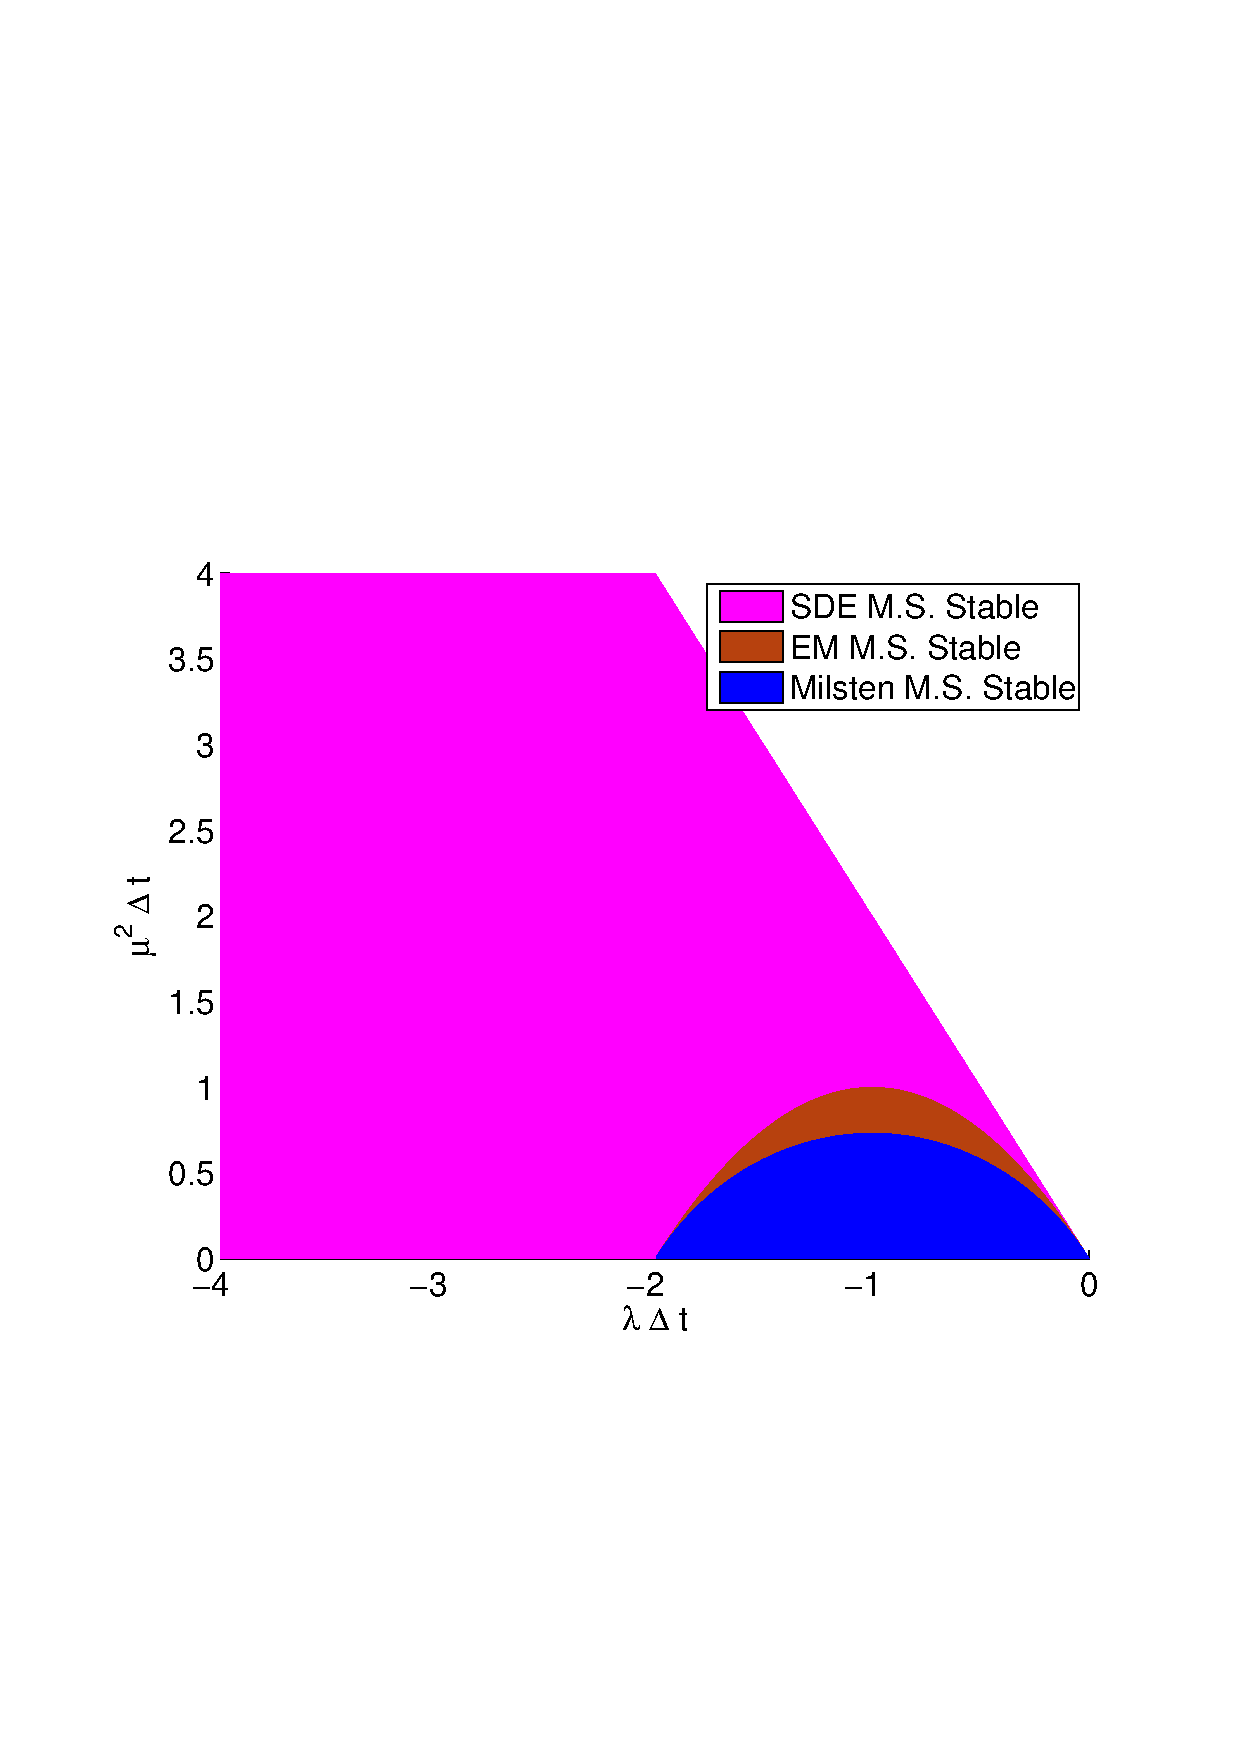
\includegraphics[scale=0.5]{Regions.pdf}
      \centering
    \end{figure}


  \clearpage
  \item % Question 4
    In this problem, I will simulate Geometric Brownian motion
    satisfying
    \begin{align}
      \label{q4.0}
      dX_t = \lambda X_t dt + \mu X_t dW_t
    \end{align}
    on the interval $t\in[0,10]$. Using the notation in (\ref{q4.0}), we
    know that this has an analytical solution
    \begin{align}
      X_t = X_0 \cdot e^{\left(\lambda-\frac{\mu^2}{2}\right) t + \mu W_t}
      \label{q4.1}
    \end{align}
    \begin{enumerate}
      \item % Question 4a
        Here, we implement Euler-Maryama for (\ref{q4.0}) when
        ($\lambda, \mu$)=(2,1).  Some sample paths at varying step sizes
        are plotting in Figure~\ref{fig:q4a}.The analytical solution is
        a solid line, while discretized paths are in dashed lines. For
        most of the step sizes, they are indistinguishable.
        \begin{figure}[htpb!]
          \caption{Sample EM Paths\label{fig:q4a}}
          \includegraphics[scale=0.8]{Q4/SamplePathsEM.pdf}
          \centering
        \end{figure}
        The relevant plot for strong convergence is shown in
        Figure~\ref{fig:q4a.1}.
        \begin{figure}[htpb!]
          \caption{Strong Convergence for EM\label{fig:q4b}}
          \includegraphics[scale=0.5]{Q4/StrongEM.pdf}
          \centering
        \end{figure}

      \item % Question 4b
        Here, we implement the Milstein scheme for
        $(\lambda,\mu)=(2,1)$.  Some sample paths at varying step sizes
        are plotting in Figure~\ref{fig:q4b}. The analytical solution is
        a solid line, while discretized paths are in dashed lines. For
        most of the step sizes, they are indistinguishable.
        \begin{figure}[htpb!]
          \caption{Sample EM Paths\label{fig:q4b}}
          \includegraphics[scale=0.8]{Q4/SamplePathsMilstein.pdf}
          \centering
        \end{figure}
        The relevant plot for strong convergence is shown in
        Figure~\ref{fig:q4b.1}.
        \begin{figure}[htpb!]
          \caption{Strong Convergence for Milstein\label{fig:q4b}}
          \includegraphics[scale=0.5]{Q4/StrongMilstein.pdf}
          \centering
        \end{figure}

    \end{enumerate}
\end{enumerate}

\clearpage
\appendix

\section{Question 1a Detail}

  In Question 1a, I chose the function $f(t,x)=tx$ in the
    application of Ito's Lemma by first considering the case of
    non-stochastic integrals. Namely, the integral we want to simplify
    \begin{align*}
      \int^t_0 s \;dW_s
    \end{align*}
    looks a lot like the following deterministic integral:
    \begin{align*}
      \int^t_0 s \;dg(s)
    \end{align*}
    Supposing that $g$ is differentiable, we could write this
    \begin{align*}
      \int^t_0 \;s dg(s)
      = \int^t_0 s g'(s) \;ds
    \end{align*}
    Using integration by parts with:
    \begin{align*}
      u = s &\quad du = ds \\
      v = g &\quad dv = g'(s) ds
    \end{align*}
    we can simplify further
    \begin{align*}
      \int^t_0 \;s dg(s)
      &= \int^t_0 s g'(s) \;ds \\
      &= \left( sg(s)\right)^t_0 - \int^t_0 g(s) \;ds \\
      &= tg(t) - \int^t_0 g(s) \;ds
    \end{align*}
    Although $W_t$ is not differentiable, so that this argument would
    not work for $g(t) = W_t$, it's at least suggestive that we might
    want to use $f(t,x) = tx$ as our function (especially since the
    steps above swapped an integral $\int^t_0 sdg(s)$ for one that is
    $\int^t_0 g(s) ds$, which will be easier to work with).

\clearpage
\section{Matlab Code}

\subsection{Discretization and Simulation}
\matlabcode{Q4/SimulateAll.m}

\clearpage
\subsection{Plotting and Calling}
\matlabcode{Q4/homework9.m}

\clearpage
\subsection{Stability Region Plot}
\matlabcode{plot_regions.m}


\end{document}


%%%%%%%%%%%%%%%%%%%%%%%%%%%%%%%%%%%%%%%%%%%%%%%%%%%%%%%%%%%%%%%%%%%%%%%%
%%%%%%%%%%%%%%%%%%%%%%%%%%%%%%%%%%%%%%%%%%%%%%%%%%%%%%%%%%%%%%%%%%%%%%%%
%%%%%%%%%%%%%%%%%%%%%%%%%%%%%%%%%%%%%%%%%%%%%%%%%%%%%%%%%%%%%%%%%%%%%%%%

%%%% SAMPLE CODE %%%%%%%%%%%%%%%%%%%%%%%%%%%%%%%%%%%%%%

    %% BIBLIOGRAPHIES %%

        \cite{LabelInSourcesFile}  %Use in text; cites
        \citep{LabelInSourcesFile} %Use in text; cites in parens

        \nocite{LabelInSourceFile} % Includes in refs w/o specific citation
        \bibliographystyle{apalike}  % Or some other style

        % To ditch the ``References'' header
        \begingroup
        \renewcommand{\section}[2]{}
        \endgroup

        \bibliography{sources} % where sources.bib has all the citation info

    %% SPACING %%

        \vspace{1in}
        \hspace{1in}


    %% INCLUDING PDF PAGE %%

        \includepdf{file.pdf}


    %% INCLUDING CODE %%

        \verbatiminput{file.ext}
            %---Includes verbatim text from the file
        \texttt{text}
            %---Renders text in courier, or code-like, font

        \matlabcode{file.m}
            %---Includes Matlab code with colors and line numbers


    %% INCLUDING FIGURES %%

        % Basic Figure with size scaling
            \begin{figure}[h!]
               \centering
               \includegraphics[scale=1]{file.pdf}
            \end{figure}

        % Basic Figure with specific height
            \begin{figure}[h!]
               \centering
               \includegraphics[height=5in, width=5in]{file.pdf}
            \end{figure}

        % Figure with cropping, where the order for trimming is  L, B, R, T
            \begin{figure}
               \centering
               \includegraphics[trim={1cm, 1cm, 1cm, 1cm}, clip]{file.pdf}
            \end{figure}


        % Side by Side figures
            \begin{figure}[h!]
                \centering
                \mbox{\subfigure{
                    \includegraphics[scale=1]{file1.pdf}
                }\quad\subfigure{
                    \includegraphics[scale=1]{file2.pdf}
                }
                }
            \end{figure}


